\chapter{Meta}

\section{Hintergrund}

Wir leben in einer Gesellschaft, in der jährlich ca. 1.3 Milliarden Tonnen an Lebensmitteln, die für den Verzehr geeignet sind, aufgrund ihrer Abweichung von Marktnormen, Überproduktion oder aufgrund ihres Haltbarkeitsdatums weggeworfen werden.

Besonders Restaurants und Hotels mit einem All-You-Can-Eat-Buffet tragen einen signifikanten Teil zu dieser enormen Verschwendung von essbaren Lebensmitteln bei.

Genau hier kommt \textbf{Sokka} ins Spiel und soll für dringend nötige Veränderung sorgen. Durch die Möglichkeit einfach Bestellungen von Kunden verwalten zu können haben Köche, die auf die Dienste von Sokka zurückgreifen, einen besseren Überblick darüber, welche Menge von welchen Gerichten zubereitet werden muss.\\
Auf diese Weise kann nachhaltig verhindert werden, dass zu viele Speisen gekocht und im Endeffekt trotz ihrer Frische entsorgt werden.

\section{Namensherkunft}

Der Name \textbf{Sokka} stammt ursprünglich aus der Serie \textit{Avatar: Der Herr der Elemente}. In jener Serie ist Sokka ein Nebencharakter, der ständig über sein konstantes Bedürfnis zu essen Kund tut und eine Vorliebe dafür hat, exotische Spezialitäten in besonders großen Mengen zu probieren.

Da sich dieses Projekt ebenso um die verschiedene Speisen und Gerichte eines Restaurants und deren Verwaltung dreht, haben wir uns dazu entschlossen, das System nach eben genannter Figur zu benennen.

\begin{figure}[H]
    \begin{center}
        
\includegraphics[width=0.25\textwidth]{images/Intro/Sokka.png}
        \caption{Der Charakter \textbf{Sokka} aus der Serie \textit{Avatar: Der Herr der Elemente}}
        \cite{nickelodeon2005}
    \end{center}
\end{figure}

\newpage

\section{Projektlogo}

Das Markenzeichen des vorher genannten Charakters \textbf{Sokka} ist sein sofort erkennbarer Bommerang. Aus diesem Grund haben wir uns dazu entschieden, eine \glqq grinsende\grqq Version dieses Boomerangs als Logo für dieses Projekt zu verwenden.

\begin{figure}[H]
    \begin{center}
        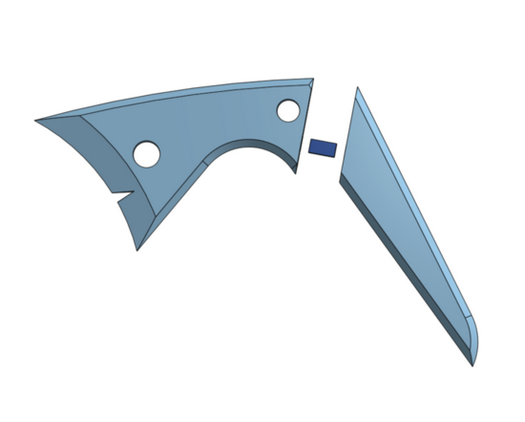
\includegraphics[width=0.25\textwidth]{images/Intro/Boomerang.png}
        \caption{Sokka's Boomerang}
        \cite{aguilar2020}
    \end{center}
\end{figure}